\section{Theory of relaxation of electromagnetic filed. Heisenberg--Langevin method}

We have discussed:
\begin{enumerate}
	\item Two-level system (e.g. atom) and one mode field. Result: Rabi oscillations.
	\item Two-level system and continuum of modes (e.g. cavity). Result: spontaneous emission.
	\item One-mode field and continuum of modes. Result: let's find out!
\end{enumerate}

\begin{figure}[h!]
	\centering
	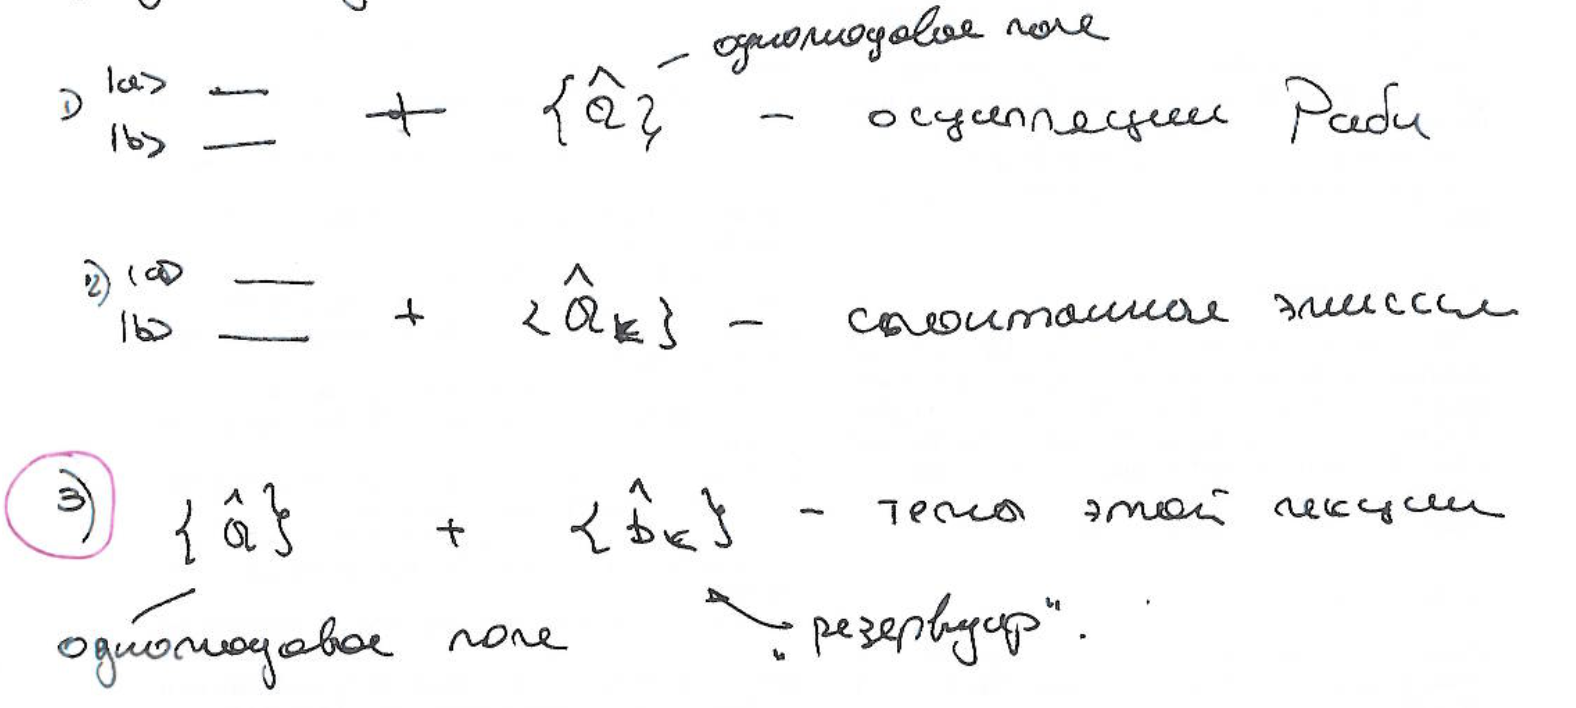
\includegraphics[width=0.8\linewidth]{fig/L9/fig1}
	\caption{Different possible cases for analytical consideration.}
	\label{fig:fig11}
\end{figure}


We are interested in dynamics of $\hat{b}(t)$ and $\hat{a}(t)$ in thermodynamics equilibrium at the temperature $T$. We consider modes which are fluctuate independently
\begin{eqnarray}
	\left \langle \hat{b}^{\dagger}_{\kv} (0) \hat{b}_{\kv'} (0) \right \rangle &=& \bar{n}_{\kv} \delta_{\vec{k}\vec{k}'}, \\
	\av{\hat{b}_{\kv}(0)} = \av{\hat{b}^{\dagger}_{\kv}(0)} &=& 0,\\
	\av{\hat{b}_{\kv} (0) \hat{b}^{\dagger}_{\kv'} (0) } &=& (\bar{n}_{\kv}+1) \delta_{\vec{k}\vec{k}'}, \\
	\av{\hat{b}_{\kv} (0) \hat{b}_{\kv'} (0) } = \av{\hat{b}^{\dagger}_{\kv} (0) \hat{b}^{\dagger}_{\kv'} (0) } &=& 0.
\end{eqnarray}
Density matrix and distribution function in thermodynamics equilibrium is given by
\begin{equation}
	\rho_R = \Pi \left( 1 - e^{- \frac{\hbar \omega_{\vec{k}}}{kT}} \right) e^{- \frac{\hbar \omega_{\vec{k}} \hat{b}_{\kv}^{\dagger} \hat{b}_{\kv}}{kT}}, \qquad \bar{n}_{\kv}  = \frac{1}{e^{\frac{\hbar \omega_{\vec{k}}}{kT}} - 1}.
\end{equation}
The Hamiltonian of the system can be written as 
\begin{equation}
	\hat{\mathcal{H}} = \underbrace{\hbar \omega \hat{a}^{\dagger} \hat{a}}_{\text{resonator}} + \underbrace{\sum_{\kv} \hbar \omega_{\kv} \hat{b}^{\dagger}_{\kv} \hat{b}_{\kv}}_{\text{cavity}} + \underbrace{\sum_{\kv} \hbar  \left( g_{\kv} \hat{b}_{\kv}^{\dagger} \hat{a}_{\kv} + g^*_{\kv} \hat{a}_{\kv}^{\dagger} \hat{b}_{\kv}  \right)}_{\hat{\mathcal{H}}_{\text{int}}}.
\end{equation}
The  explicit form of $g_{\kv}$ is strongly depend on exact system. However we know the asymptotic behavior --- if the resonator is ideal then $g_{\kv} = 0$.

Time evolution is defined by
\begin{equation}
	\hat{\dot{a}}(t) = \frac{i}{\hbar} \left[ \hat{\mathcal{H}}, \hat{a}  \right], \qquad  	\hat{\dot{b}}(t) = \frac{i}{\hbar} \left[ \hat{\mathcal{H}}, \hat{b}  \right],
\end{equation} 
which gives 
\begin{numcases}{}
		\hat{\dot{a}}(t) = -i \omega \hat{a}(t) - i \sum_{\kv} g_{\kv}^* \hat{b}_{\kv}(t), \label{eq:a_dyn}\\
		\hat{\dot{b}}_{\kv}(t) = -i \omega_{\kv} \hat{b}_{\kv}(t) - i  g_{\kv} \hat{a}(t),
		\label{eq:b_dyn}
\end{numcases}
Important to notice that it is sensible to consider only the mean values of operators. 

Now let us solve this system. it is easy to verify that the solution of  \eqref{eq:b_dyn}  is
\begin{equation}
	\hat{b}_{\kv}(t) = \underbrace{\hat{b}_{\kv}(0) e^{-i\omega_{\kv} t}}_{\text{reservoir modes evolution}} - \underbrace{i g_{\kv} \int \limits_0^{t} d\tau \hat{a}(\tau) e^{-i\omega_{\kv}(t - \tau)}}_{\text{interaction between reservoir and oscillator}}
\end{equation}
then we substitute this result in \eqref{eq:a_dyn} and obtain
\begin{equation}
	\hat{\dot{a}}(t) = - i \omega \hat{a}(t) - \hat{f}_a(t) + \sum_{\kv} \left| g_{\kv} \right|^2 \int \limits_0^td\tau \hat{a}(\tau) e^{-i\omega_{\kv}(t - \tau)},
\end{equation}
where
\begin{equation}
	\hat{f}_a(t) \myeq i \sum_{\kv} g_{\kv}^* \hat{b}_{\kv}(0) e^{-i\omega_{\kv} t}
\end{equation}
is a stochastic operator as the number of photons in a particular time moment is undefined. After that we introduce 
\begin{equation}
	\hat{\tilde{a}}(t) \myeq \hat{a} e^{i \omega t}, \qquad \hat{F}_{\tilde{a}} (t) = \hat{f}_a(t) e^{i \omega t}
\end{equation}
and obtain \textit{a stochastic integro-differential equation} 
\begin{equation}
	\hat{\dot{\tilde{a}}}(t) = \sum_{\kv} \left| g_{\kv} \right|^2 \int \limits_0^t d\tau \hat{\tilde{a}} e^{i(\omega-\omega_{\kv})(t - \tau)} + \hat{F}_{\tilde{a}} (t).
	\label{eq:st_int_dif}
\end{equation}
which is quite hard to solve.

To find a solution of \eqref{eq:st_int_dif} we, first of all, make transition from sum to the integral
\begin{equation}
	\sum_{\kv} \left| g_{\kv} \right|^2 \quad \to \quad \frac{V}{\pi^2 c^3} \int \limits_0^{\infty} d \omega_{\kv} \omega_{\kv}^2 \left| g_{\omega_{\kv}} \right|^2.
\end{equation}
Now let us consider only the integral in \eqref{eq:st_int_dif} which becomes
\begin{multline}
	\frac{V}{\pi^2 c^3} \int \limits_0^{\infty} d \omega_{\kv} \omega_{\kv}^2 \left| g_{\omega_{\kv}} \right|^2 \int \limits_0^t d\tau \hat{\tilde{a}}(\tau)e^{i(\omega - \omega_{\kv})(t - \tau)} = \\ =\Bigg/ \omega_{\kv}^2 \left| g_{\omega_{\kv}} \right|^2 \text{ is a slow function} \Bigg/
	\approx \frac{V}{\pi^2 c^3} \int \limits_0^t d \tau \hat{\tilde{a}}(\tau) \cdot \omega_{\kv}^2 \left| g_{\omega_{\kv}} \right|^2 \cdot  \underbrace{\int \limits_0^{\infty} d \omega_{\kv} e^{i(\omega - \omega_{\kv})(t - \tau)}}_{\hookrightarrow\approx 2\pi \delta(t - \tau)} =\\= \frac{V}{\pi^2 c^3} \omega_{\kv}^2 \cdot 2 \pi \left| g_{\omega_{\kv}} \right|^2 \underbrace{\int \limits_0^t d\tau \hat{\tilde{a}}(\tau) \delta(t - \tau)}_{\half \hat{\tilde{a}}(t)}  =\frac{\Gamma}{2}\hat{\tilde{a}}(t),
\end{multline}
where we defined a relaxation constant $\Gamma$ and density of states $D$:
\begin{equation}
	\Gamma \myeq D(\omega_{\kv}) \cdot 2 \pi \left| g_{\omega_{\kv}} \right|^2  , \qquad D(\omega_{\kv}) = \frac{V \omega_{\kv}^2}{\pi^2 c^3} = \int d^3 r \rho(\vec{r}, \omega_{\kv}).
\end{equation}
So finally 
\begin{equation}
	\boxed{\hat{\dot{\tilde{a}}}(t) = - \frac{\Gamma}{2} \hat{\tilde{a}}(t) + \hat{F}_{\tilde{a}} (t). }
\end{equation}

\textit{Remark:} we could obtain the same result if we would have considered the dynamics of atom's operator $\hat{\dot{\sigma}}_z(t)$.

\begin{testexample}[Connection between dissipation and fluctuation]
	Let us put $\hat{F}_{\tilde{a}} (t) = 0$. It means that $\hat{\tilde{a}}(t) = \hat{\tilde{a}}(0) e^{- \frac{\Gamma}{2} t}$ which leads to
	\begin{equation}
		\left[ \hat{\tilde{a}}(t), \hat{\tilde{a}}^{\dagger}(t) \right] = e^{- \Gamma t} \neq 1.
	\end{equation}
	That is nonsense! It couldn’t be, so we can not just put the stochastic term to zero. \textit{If there is a dissipation then there have to be fluctuation in the system.}
\end{testexample}


